\documentclass{article}
\usepackage[a4paper, total={6.5in, 9in}]{geometry}
\usepackage{breakurl}
\usepackage{amsmath}
\usepackage{amssymb}
\usepackage{caption}
\usepackage{graphicx}
\usepackage{hyperref}
\usepackage{subfig}
\usepackage{booktabs}
\usepackage{multirow}
\usepackage{longtable}
\usepackage{array}
\usepackage{xcolor}
\hypersetup{
    colorlinks=true,
    linkcolor=blue,
    filecolor=magenta,
    urlcolor=cyan,
    pdftitle={PREDICT-AML Supplementary},
    pdfpagemode=FullScreen,
}

\begin{document}

\title{PREDICT-AML: Personalized REsponse via Drug Interaction and Cellular Traits for Acute Myeloid Leukemia\\[1ex]
\large Supplementary Information}
\author{Mohammed Al-Ani, Siddhi P. Jani, Halima Bensmail, Raghvendra Mall}
\date{}
\maketitle

\setcounter{figure}{0}
\renewcommand{\thefigure}{S\arabic{figure}}
\setcounter{table}{0}
\renewcommand{\thetable}{S\arabic{table}}

%% ──────────────────────────────────────────────────────────────────────────
\section*{Supplementary Figures}
\vspace{-5mm}
%% Fig S1 ─ RNA-seq QC
\begin{figure}[!ht]
    \centering
    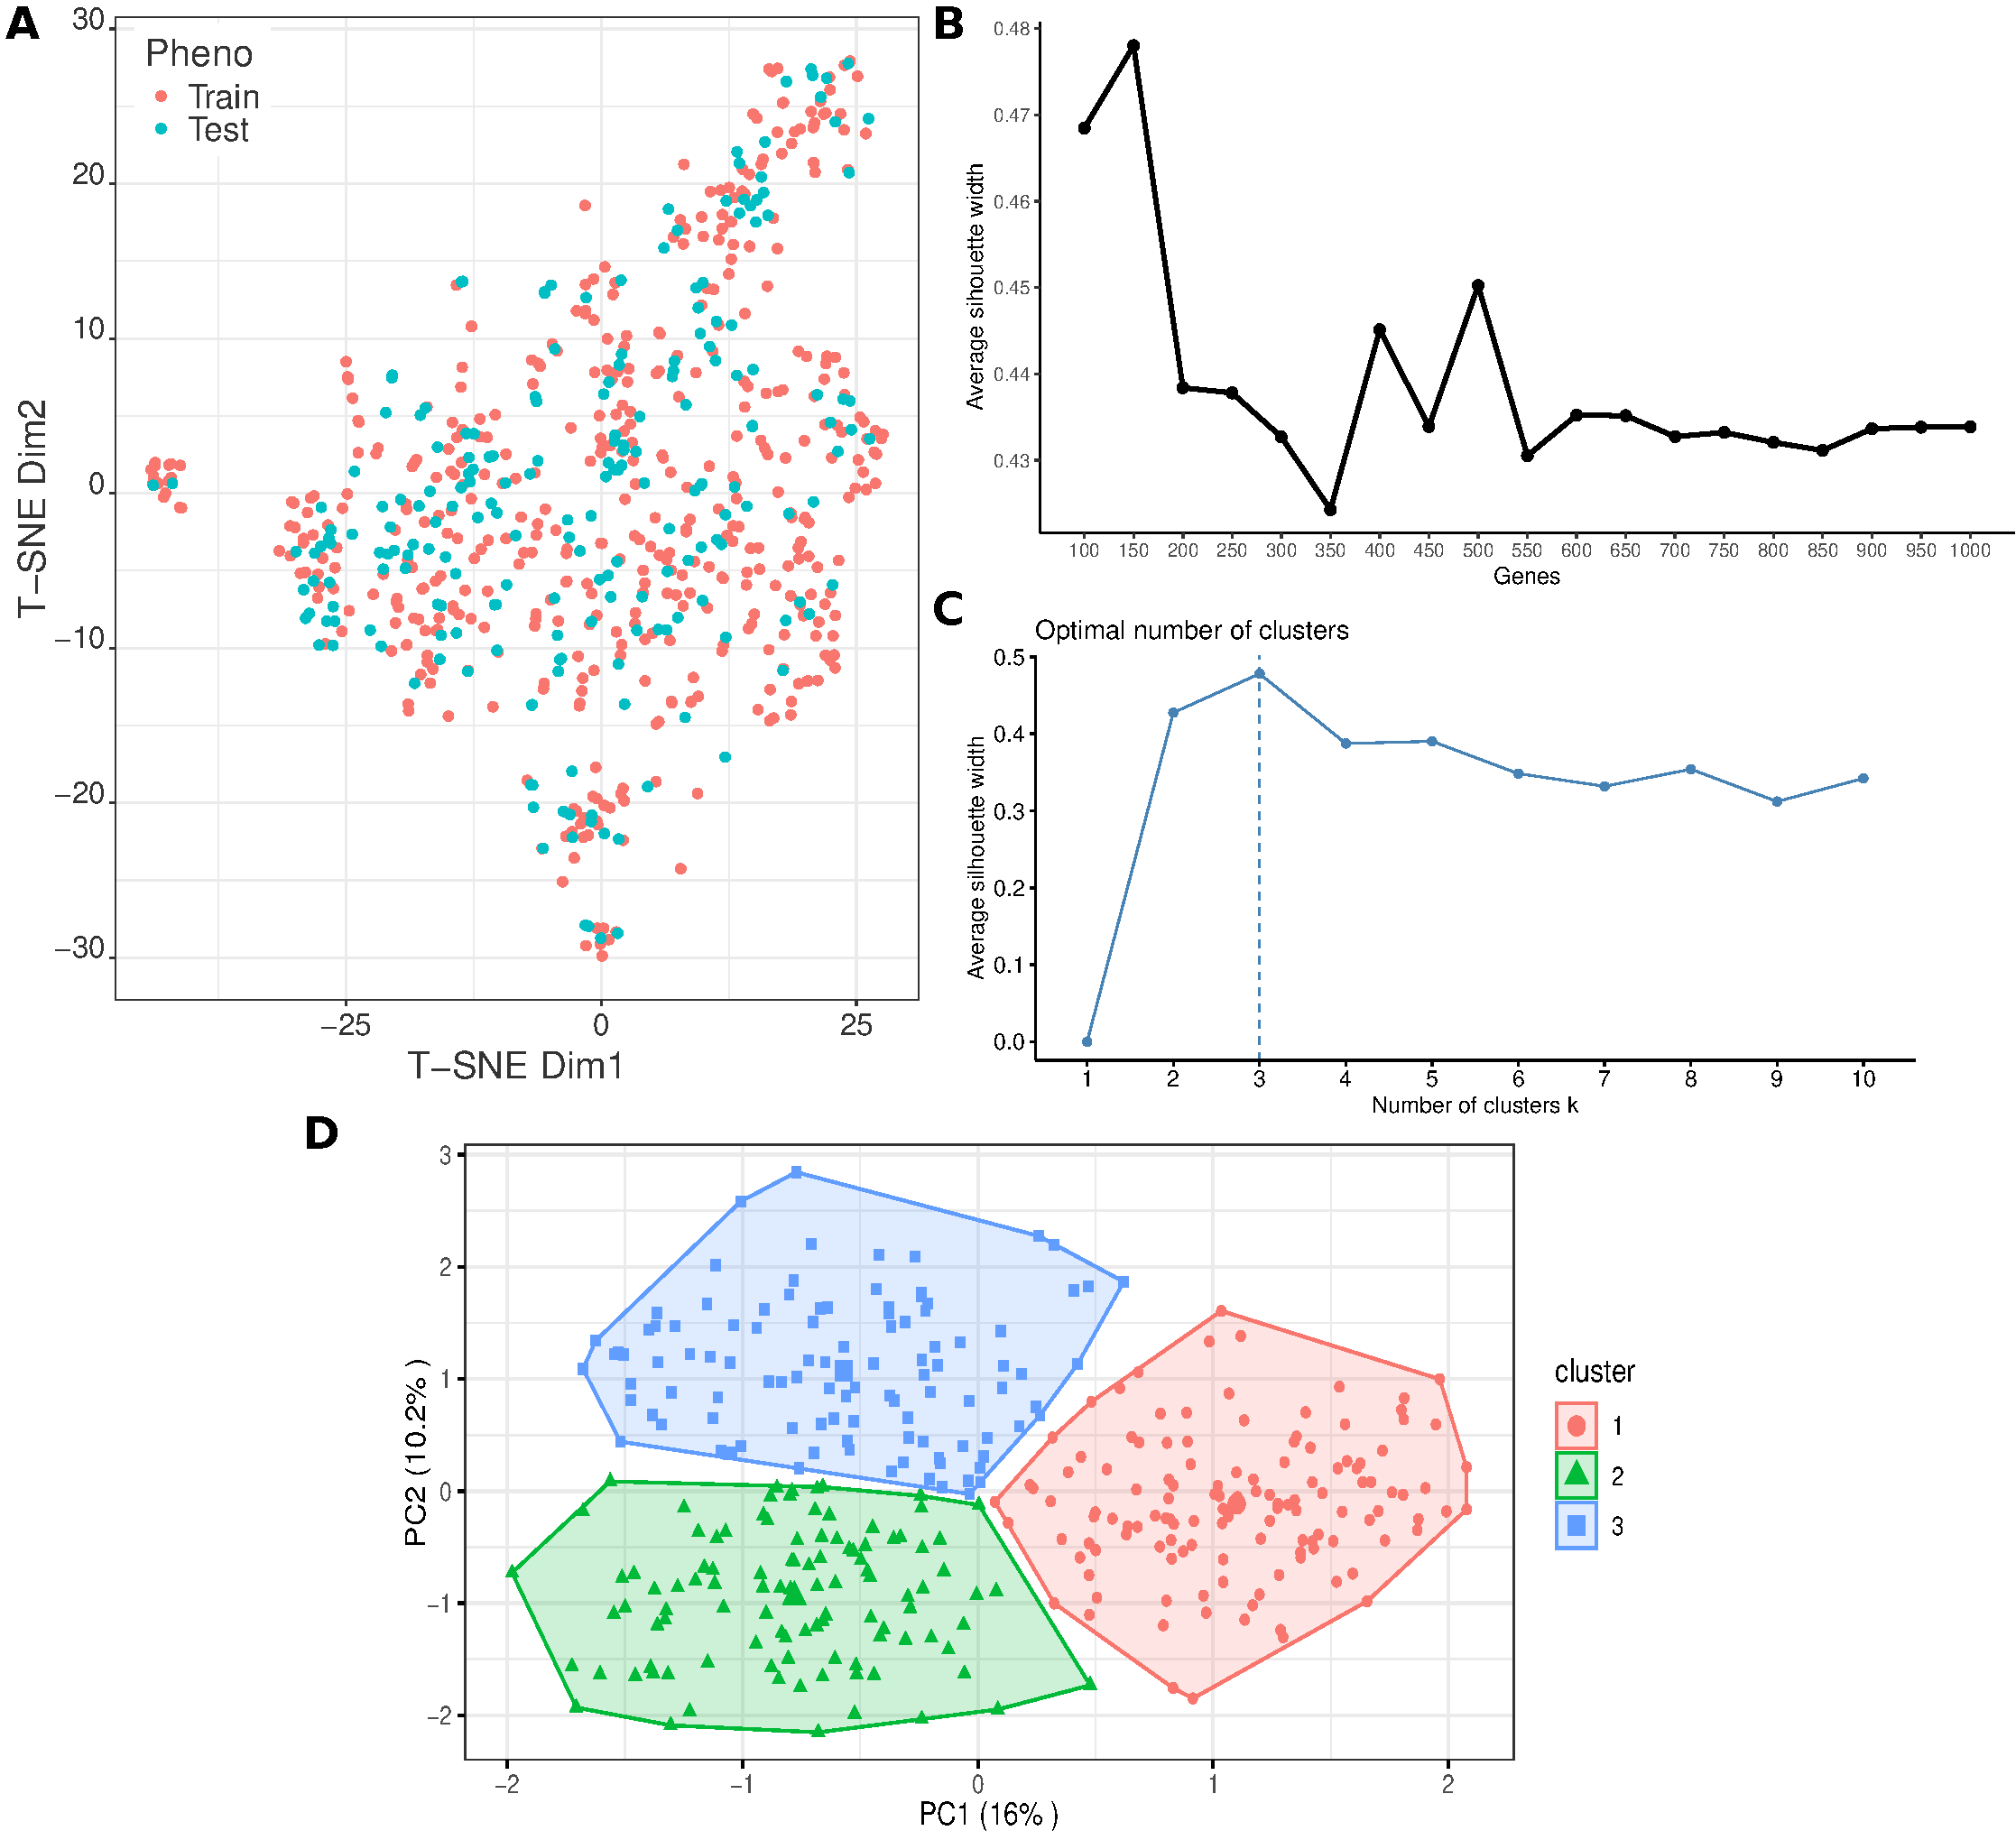
\includegraphics[width=0.88\textwidth]{figures/Supp_Fig1.pdf}
    \caption{\textbf{Transcriptomic quality control and unsupervised clustering of BeatAML patient samples.}
    \textbf{A.}~t-SNE visualization of RNA-seq expression profiles showing a uniform, unsegregated distribution
    of training (Waves~1+2) and test (Waves~3+4) samples, confirming effective normalization and quality control.
    \textbf{B.}~Silhouette scores for unsupervised clustering using 100-1{,}000 most variable genes, with peak
    performance at 150 genes.
    \textbf{C.}~Cluster stability across $k = 2$-$10$ revealing an optimal partition of $k = 3$ transcriptional
    subgroups.
    \textbf{D.}~PCA visualization of patient samples colored by the three identified transcriptional subgroups.}
    \label{fig:suppfig1}
\end{figure}

%% Fig S2 ─ Drug vs Patient normalized prediction heatmap
\begin{figure}[!ht]
    \centering
    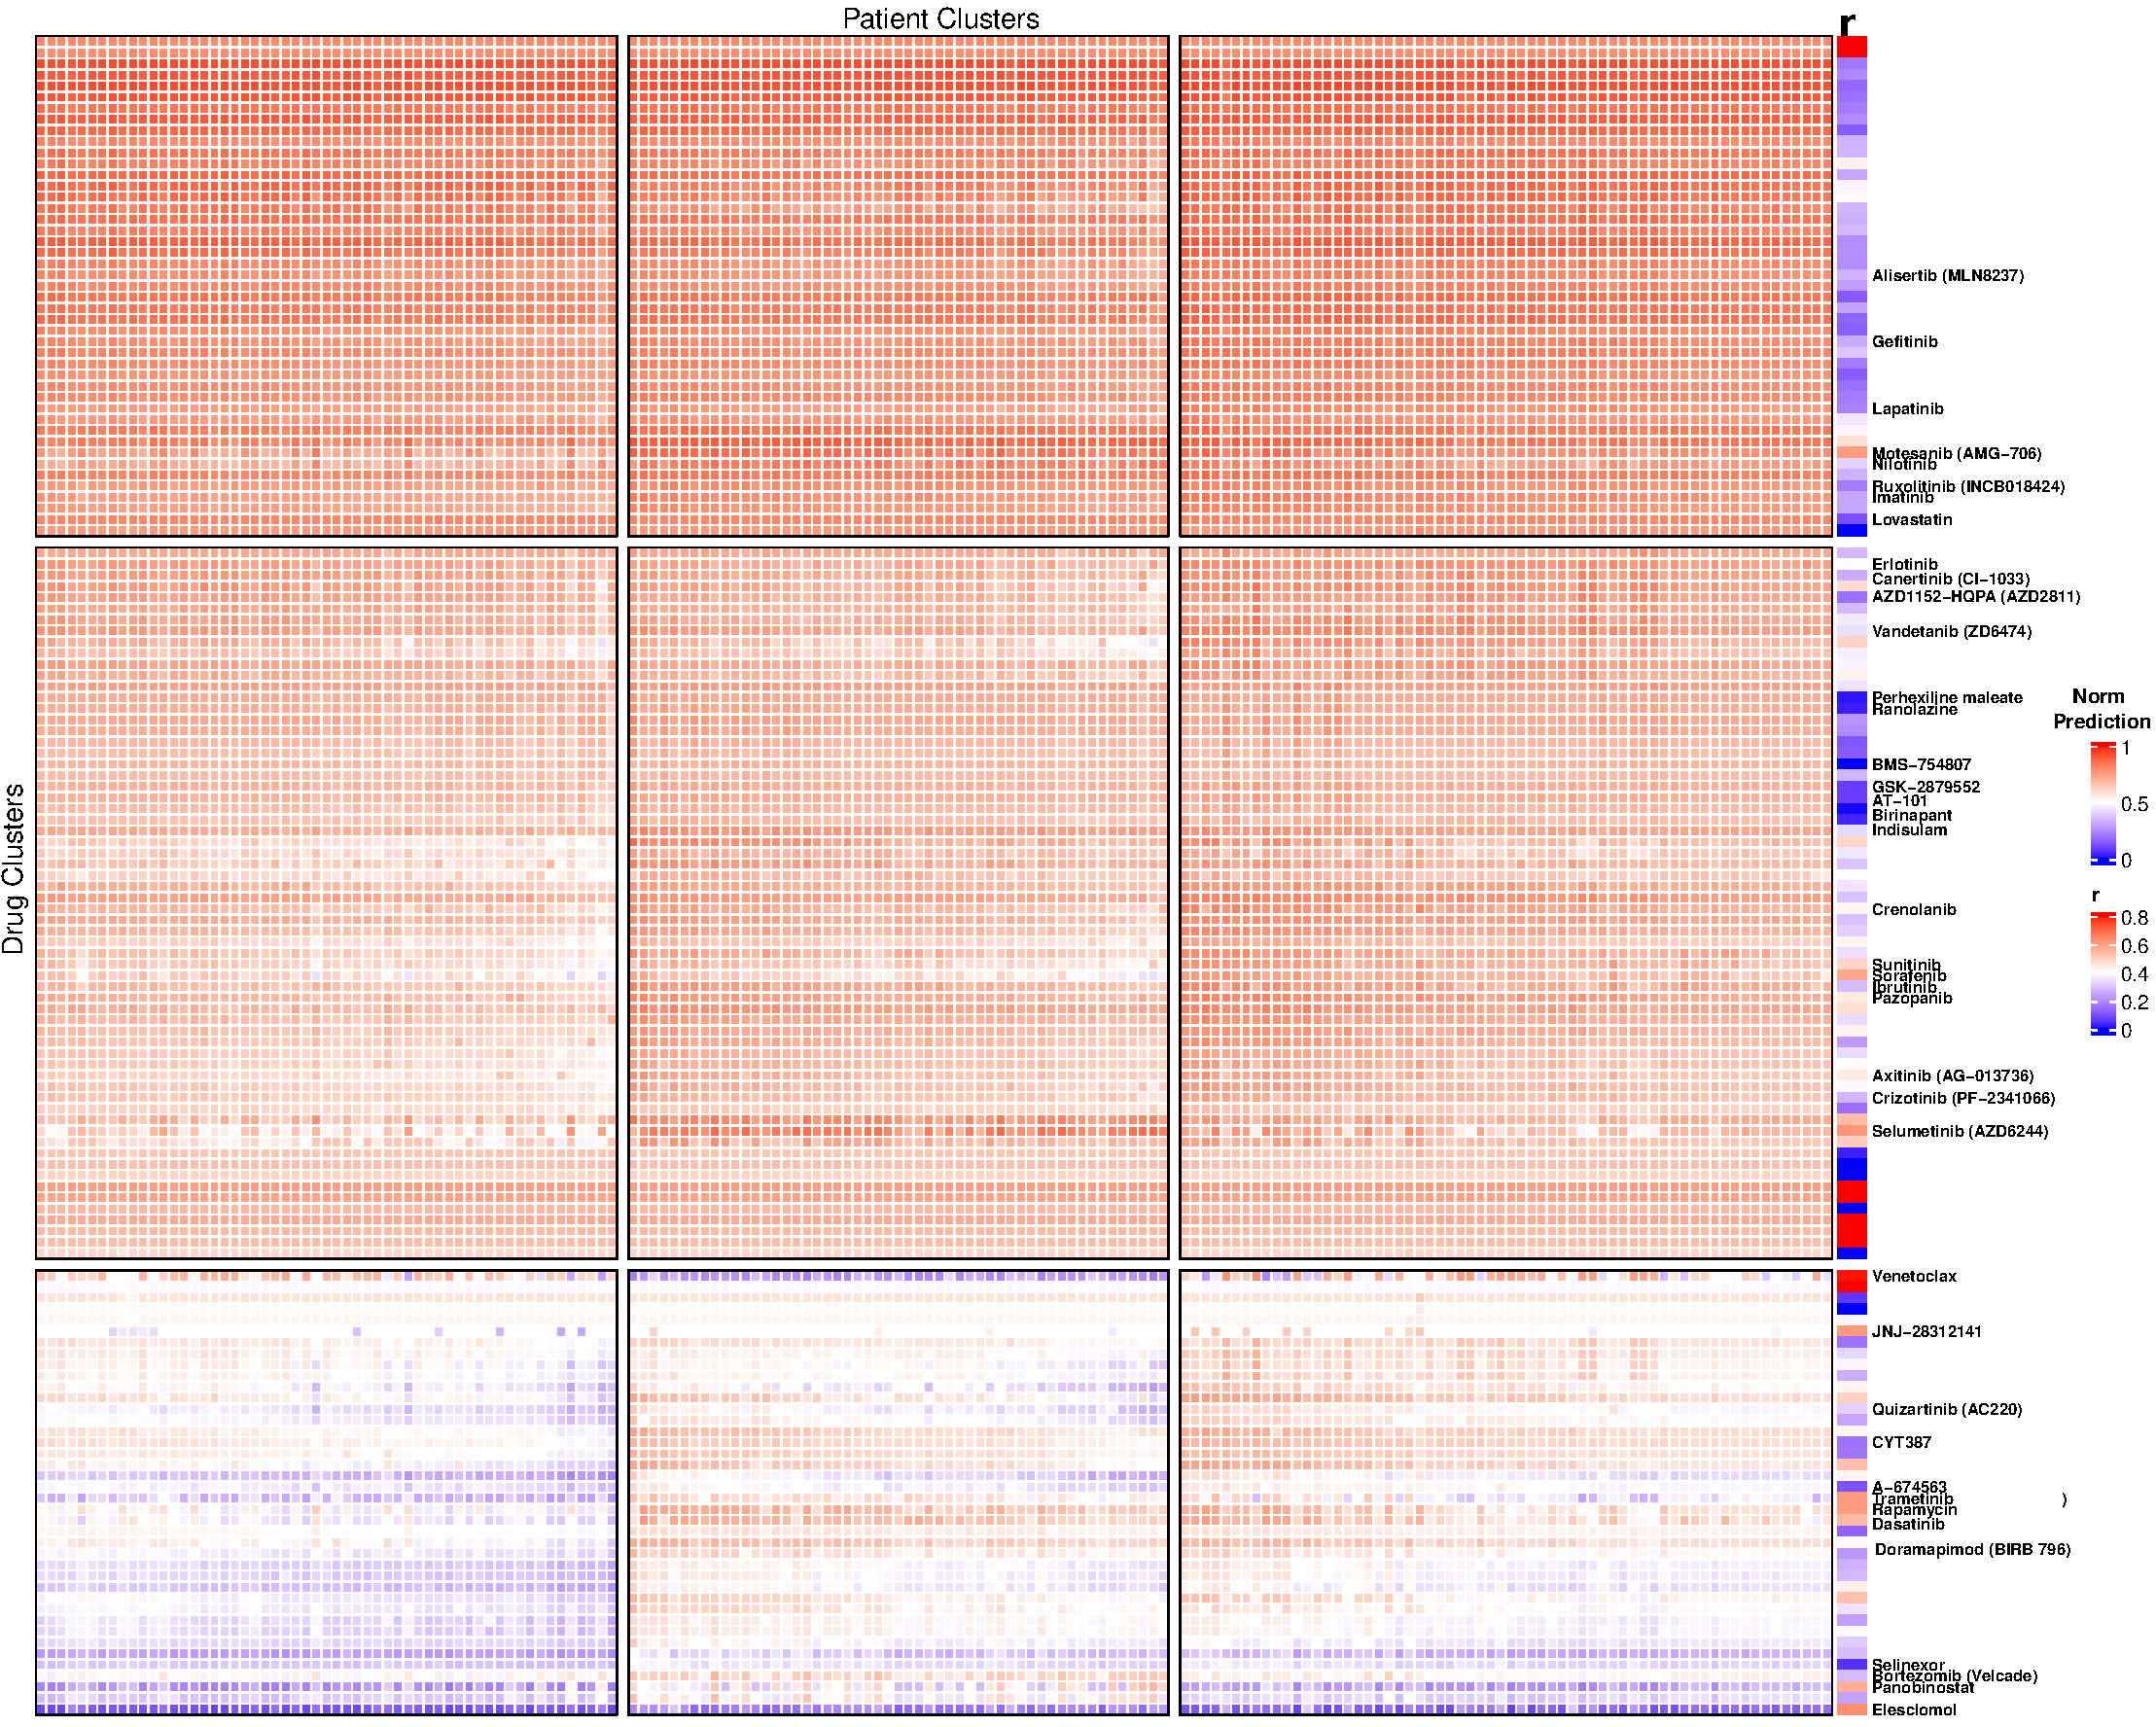
\includegraphics[width=0.97\textwidth]{../Results/Figures/Drug_vs_Patient_NormalizedPrediction_Heatmap.pdf}
    \caption{\textbf{Normalized drug response predictions across BeatAML patient samples and inhibitors.}
    Each cell encodes the normalized predicted AUC for a given drug--patient pair (z-scored per drug).
    Rows correspond to inhibitors and columns to patient samples from the BeatAML training set (Waves~1+2).
    Hierarchical clustering on both axes reveals drug clusters reflecting mechanistic class similarity and
    patient clusters corresponding to transcriptional subgroups identified in Supplementary Fig.~1.
    This landscape illustrates the heterogeneity of predicted drug sensitivity across the cohort and
    supports the patient-stratified evaluation as the clinically relevant benchmark.}
    \label{fig:suppfig2}
\end{figure}

%% Fig S3 ─ Top-20 feature importances for tree-based models
\begin{figure}[!ht]
    \centering
    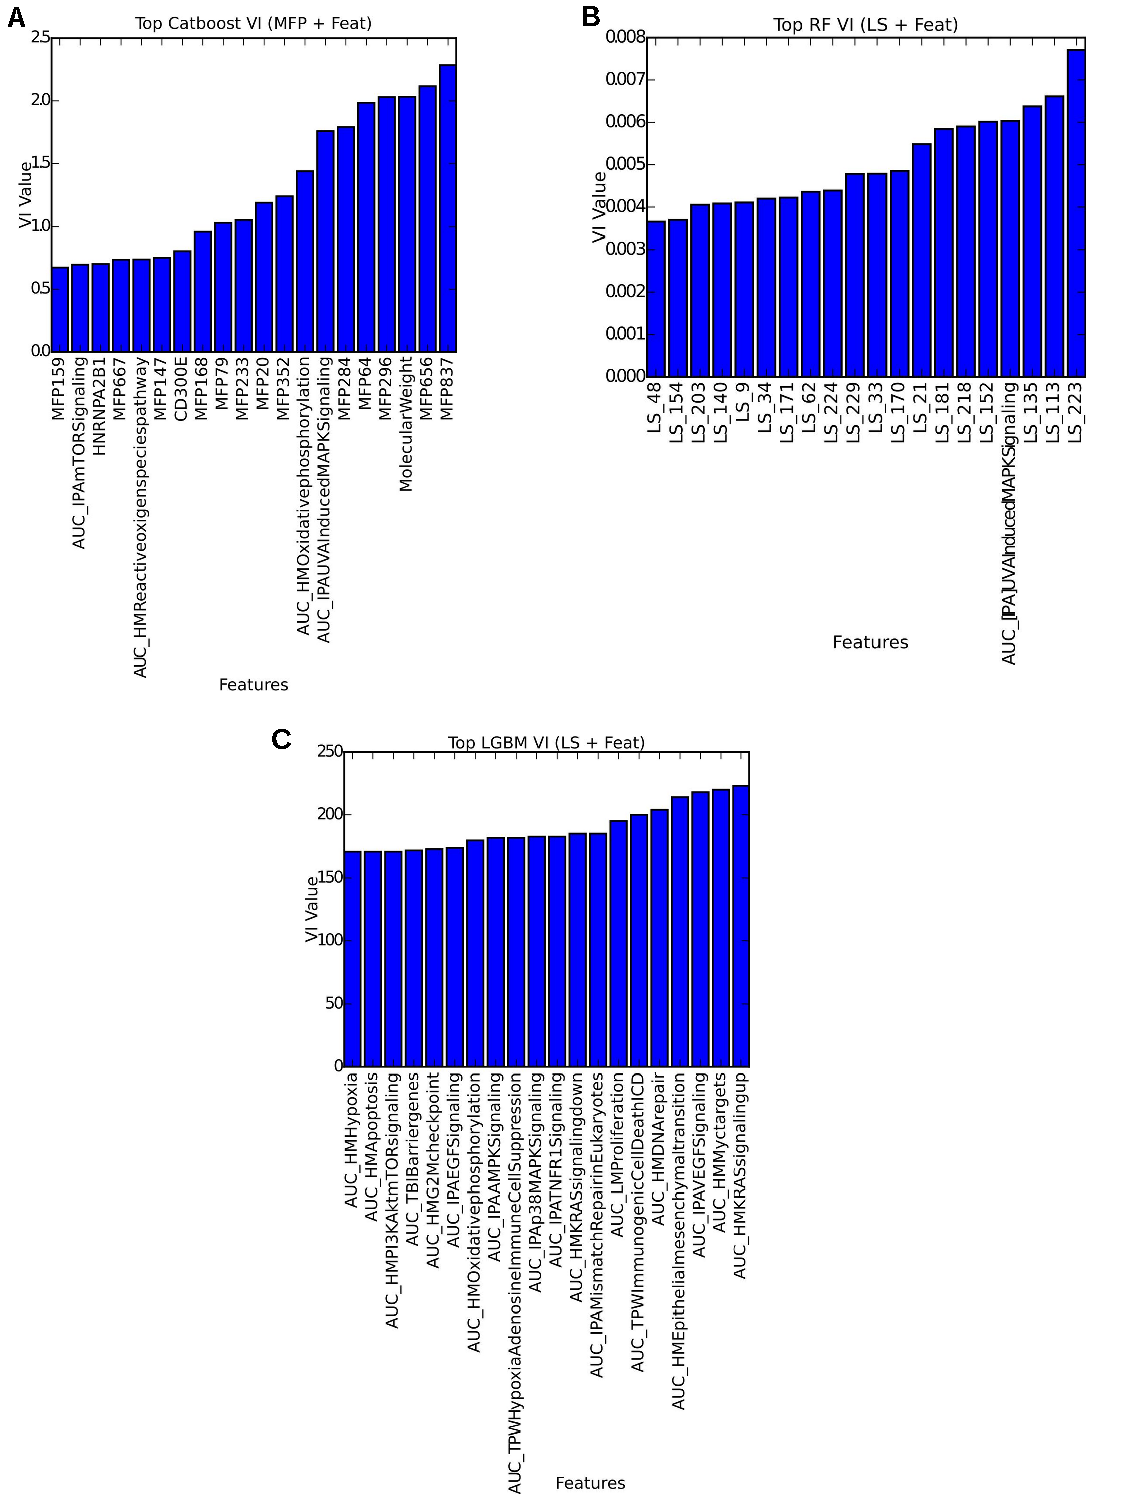
\includegraphics[width=0.97\textwidth]{jtrm_images/Supp_Fig3.pdf}
    \caption{\textbf{Top-20 most important variables for the best-performing tree-based models.}
    Feature importances are shown for CatBoost (MFP + all molecular features), Random Forest (RF), and
    LightGBM (LGBM), each using either Morgan fingerprint (MFP) or SMILES-LS embedding (LS) drug
    representations combined with the full molecular patient feature set (Feat).
    Drug--pathway AUC proximity features and transcriptomic variables consistently rank among the top
    predictors across all three models.}
    \label{fig:suppfig3}
\end{figure}

%% Fig S4 ─ TabPFN ablation baseline scatter plots
\begin{figure}[!ht]
    \centering
    \subfloat[Only\_PC Baseline][Predicted vs.\ observed AUC for the TabPFN baseline (all feature groups) with
    Only\_PC drug representation under patient-stratified CV.]{
        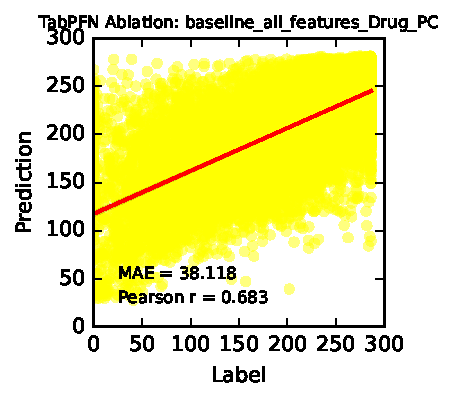
\includegraphics[width=0.85\textwidth]{figures/ablation_baseline_PC.pdf}
    }
    \qquad
    \subfloat[SMILES-LS Baseline][Predicted vs.\ observed AUC for the TabPFN baseline (all feature groups) with
    SMILES-LS (Embed) drug representation under patient-stratified CV.]{
        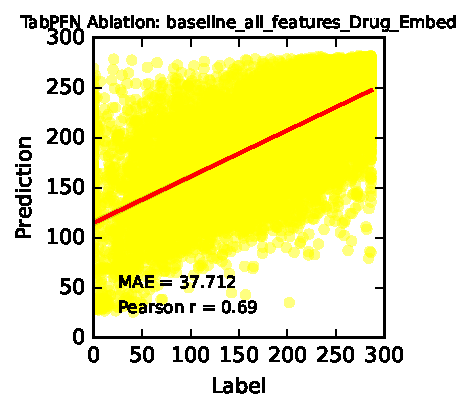
\includegraphics[width=0.85\textwidth]{figures/ablation_baseline_Embed.pdf}
    }
    \qquad
    \subfloat[PC+Embed Baseline][Predicted vs.\ observed AUC for the TabPFN baseline (all feature groups) with
    combined PC+Embed drug representation under patient-stratified CV.]{
        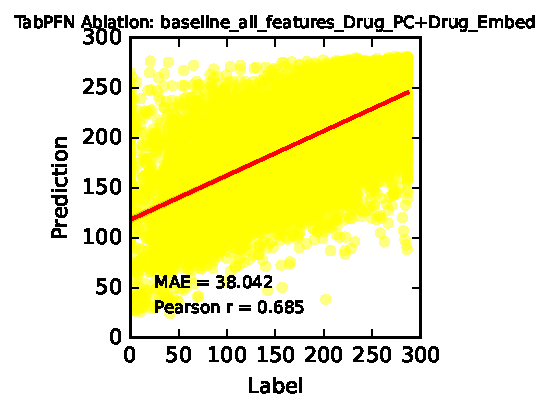
\includegraphics[width=0.85\textwidth]{figures/ablation_baseline_PC_Embed.pdf}
    }
    \caption{\textbf{TabPFN ablation study: baseline (all feature groups) prediction scatter plots.}
    Each panel corresponds to a different drug molecular representation using the full patient feature set
    (gene expression, mutation, pathway, cell-state/module features) under patient-stratified CV.
    See Supplementary Table~S2 for complete ablation results across all CV strategies and feature group
    combinations.}
    \label{fig:suppfig4}
\end{figure}

%% Fig S5 ─ LeeAML best configuration scatter
\begin{figure}[!ht]
    \centering
    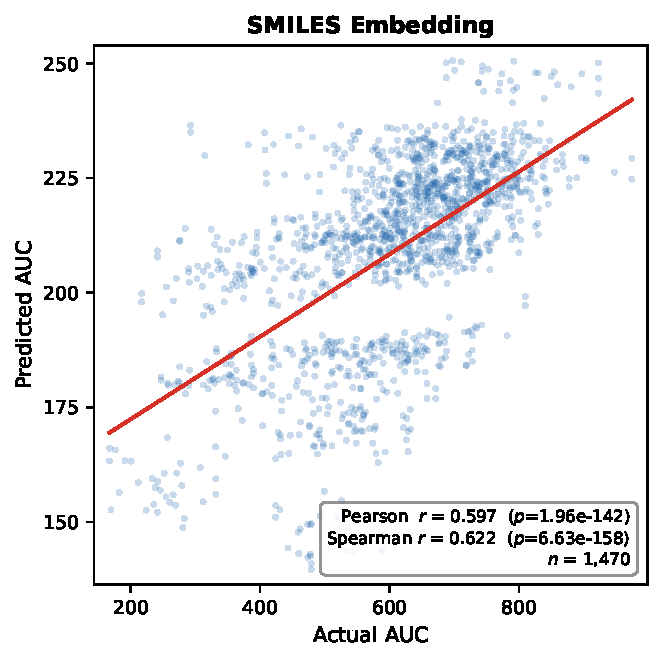
\includegraphics[width=0.85\textwidth]{figures/LeeAML_best_config_scatter.pdf}
    \caption{\textbf{External validation on LeeAML cohort: best-performing configuration (SMILES-LS).}
    Predicted vs.\ observed AUC values for the SMILES-LS (Embed) drug representation on the 49 drugs
    common between BeatAML and LeeAML ($n = 30$ patients).
    The diagonal indicates perfect prediction; color encodes drug identity.
    The SMILES-LS configuration achieves the most consistent patient-level rank correlations among all
    four drug representations evaluated on this cohort.}
    \label{fig:suppfig5}
\end{figure}

%% Figs S6–S9 ─ Individual FIMM-AML configuration scatters
\begin{figure}[!ht]
    \centering
    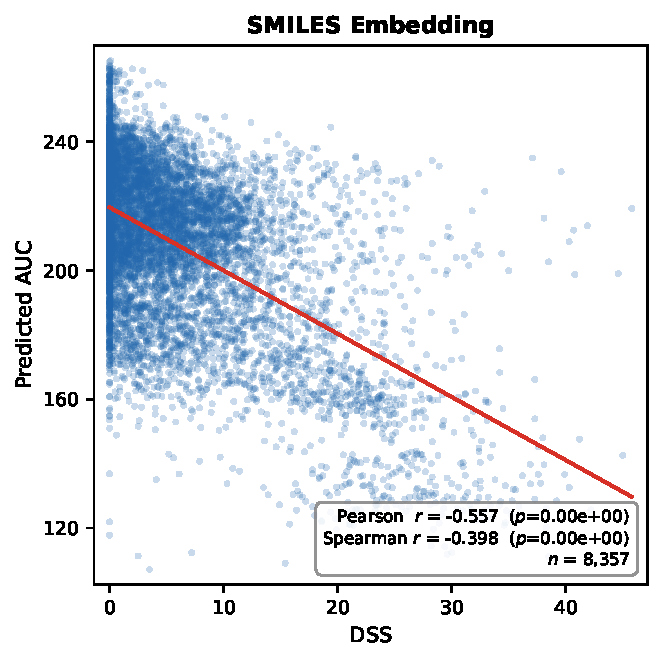
\includegraphics[width=0.82\textwidth]{figures/FIMMAML_Embed_scatter.pdf}
    \caption{\textbf{External validation on FIMM-AML cohort: SMILES-LS (Embed) drug representation.}
    Predicted AUC (BeatAML scale) vs.\ observed DSS values for the SMILES-LS drug representation on the
    78 drugs common between BeatAML and FIMM-AML ($n = 187$ patient samples).
    Spearman rank correlation is used to account for the non-linear relationship between the AUC and DSS
    drug sensitivity metrics.}
    \label{fig:suppfig6}
\end{figure}

\begin{figure}[!ht]
    \centering
    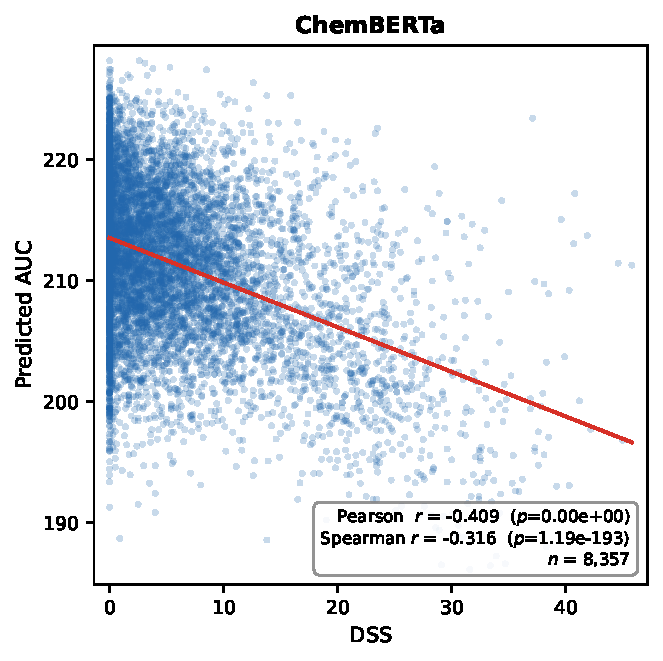
\includegraphics[width=0.82\textwidth]{figures/FIMMAML_ChemBERTa_scatter.pdf}
    \caption{\textbf{External validation on FIMM-AML cohort: ChemBERTa drug representation.}
    Predicted AUC (BeatAML scale) vs.\ observed DSS values for the ChemBERTa drug representation on the
    78 common drugs ($n = 187$ patient samples).}
    \label{fig:suppfig7}
\end{figure}

\begin{figure}[!ht]
    \centering
    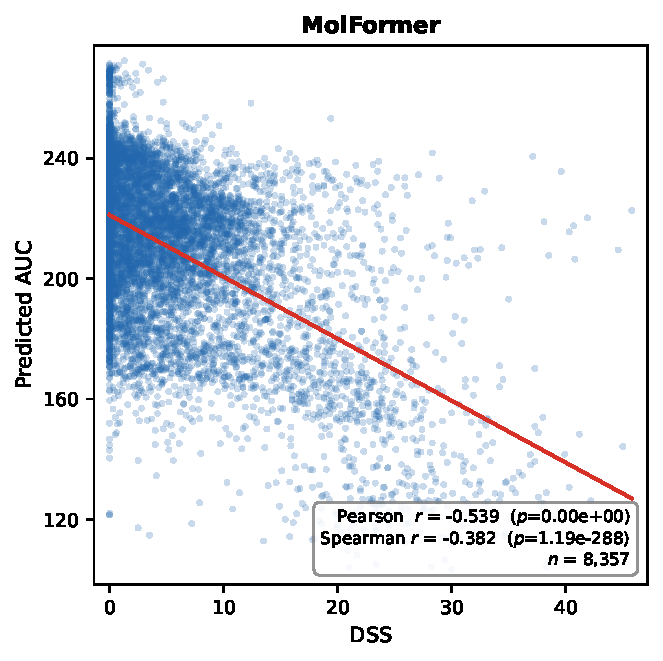
\includegraphics[width=0.82\textwidth]{figures/FIMMAML_MolFormer_scatter.pdf}
    \caption{\textbf{External validation on FIMM-AML cohort: MolFormer drug representation.}
    Predicted AUC (BeatAML scale) vs.\ observed DSS values for the MolFormer drug representation on the
    78 common drugs ($n = 187$ patient samples).}
    \label{fig:suppfig8}
\end{figure}

\begin{figure}[!ht]
    \centering
    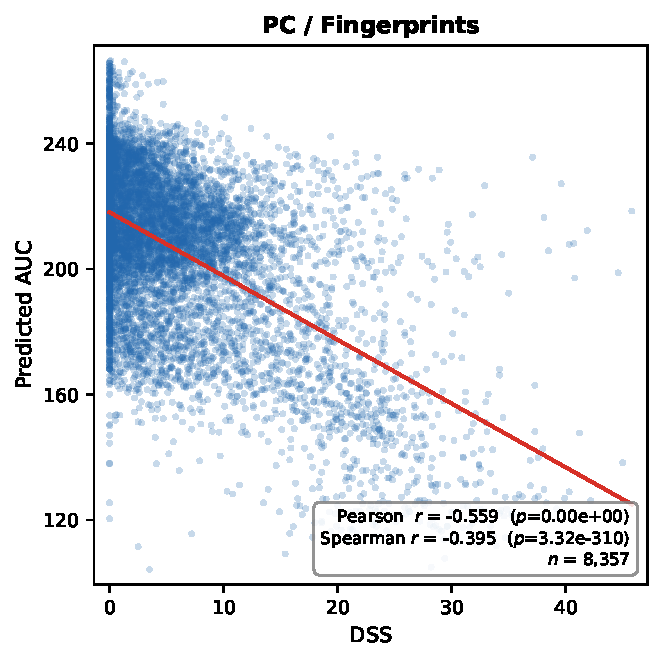
\includegraphics[width=0.82\textwidth]{figures/FIMMAML_PC_scatter.pdf}
    \caption{\textbf{External validation on FIMM-AML cohort: Only\_PC drug representation.}
    Predicted AUC (BeatAML scale) vs.\ observed DSS values for the Only\_PC (physicochemical + Morgan
    fingerprints) drug representation on the 78 common drugs ($n = 187$ patient samples).}
    \label{fig:suppfig9}
\end{figure}

%% Fig S10 ─ Full ML/DL benchmark visual
\begin{figure}[!ht]
    \centering
    \includegraphics[width=0.97\textwidth]{jtrm_images/Supp_Fig2.pdf}
    \caption{\textbf{Benchmarking of machine learning and deep learning models on the BeatAML test set.}
    \textbf{A--G.}~Scatter plots of predicted vs.\ observed AUC for the best-performing instance of each
    model class (GLR, SVR, RF, XGBoost, LightGBM, CatBoost, FFNN, CNN, LSTM, GAT, GCN) on the held-out
    Waves~3+4 test set.
    \textbf{H--S.}~Performance comparison of different combinations of patient feature sets and drug
    representations within the CatBoost framework.
    Numerical results for the full benchmark are provided in Supplementary Table~S1.}
    \label{fig:suppfig10}
\end{figure}

%% Fig S11 ─ CatBoost SHAP summary
\begin{figure}[!ht]
    \centering
    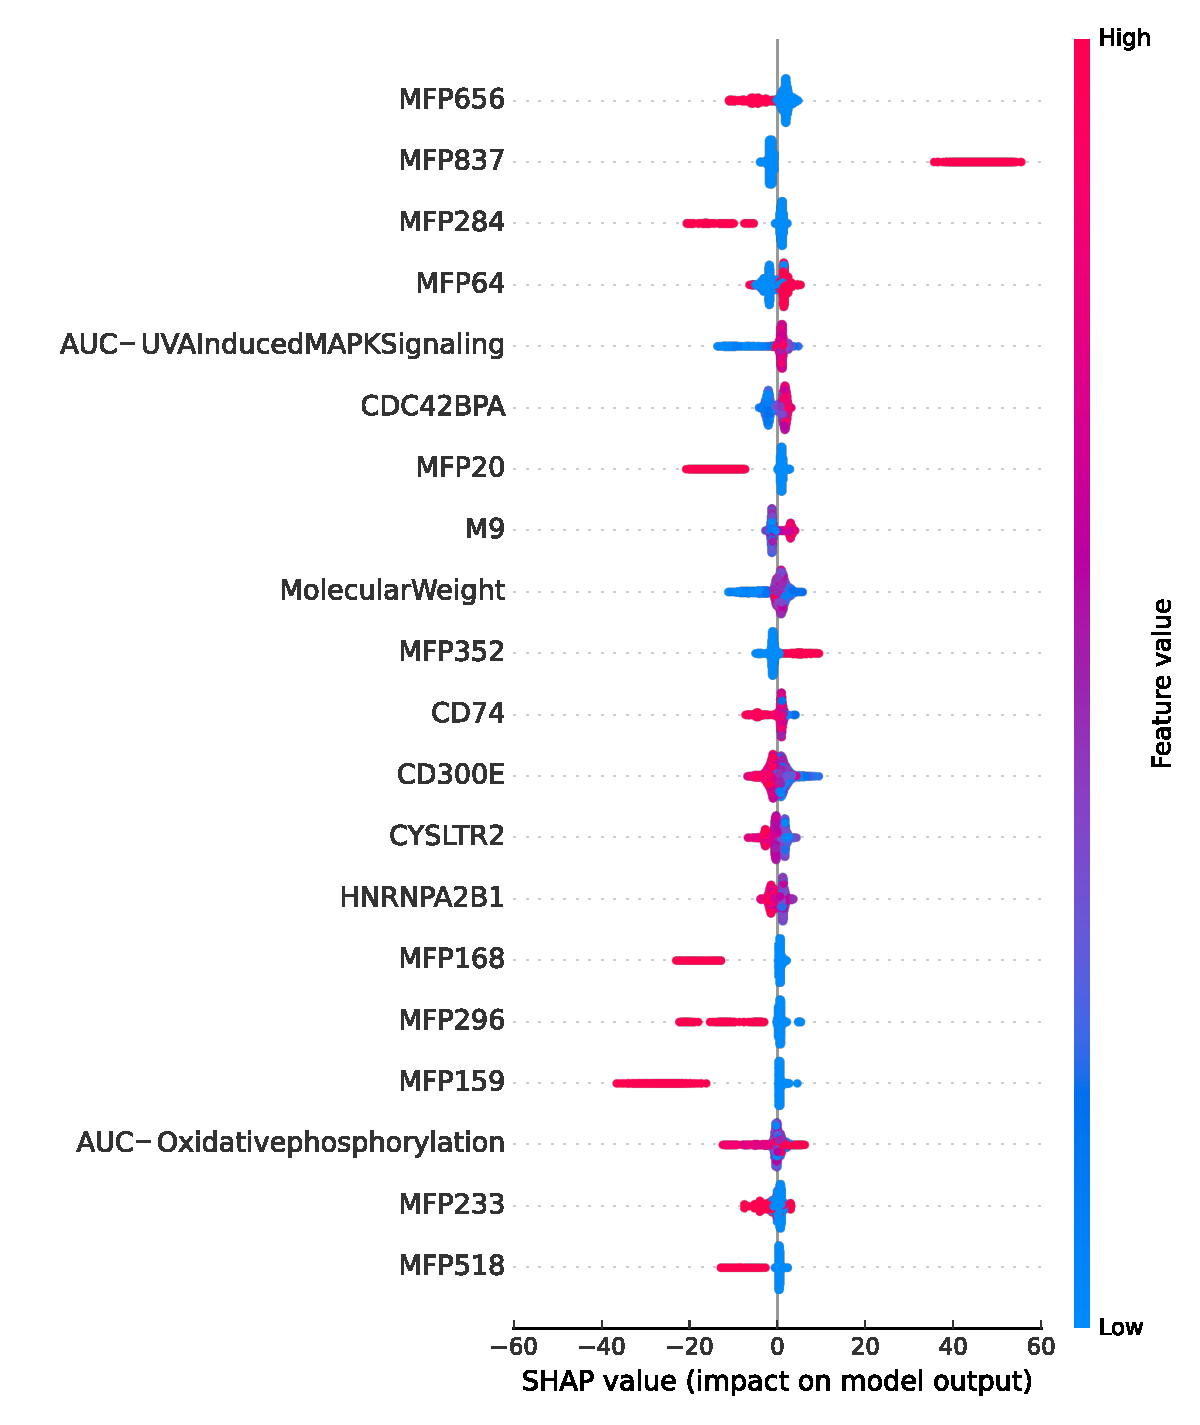
\includegraphics[width=0.82\textwidth]{jtrm_images/CatBoost_SHAP_Summary.pdf}
    \caption{\textbf{SHAP summary plot for the best CatBoost model.}
    Each row represents a feature; each point a patient--drug pair.
    Point color encodes feature value (red = high, blue = low); horizontal position indicates the SHAP value
    (contribution to predicted AUC).
    Drug--pathway proximity scores and high-variance transcriptomic features contribute most to predicted
    drug sensitivity.}
    \label{fig:suppfig11}
\end{figure}

%% Fig S12 ─ CatBoost SHAP waterfall plots
\begin{figure}[!ht]
    \centering
    \subfloat[Sensitive Sample 1][SHAP waterfall for a drug-sensitive patient--drug pair (high predicted AUC).]{
        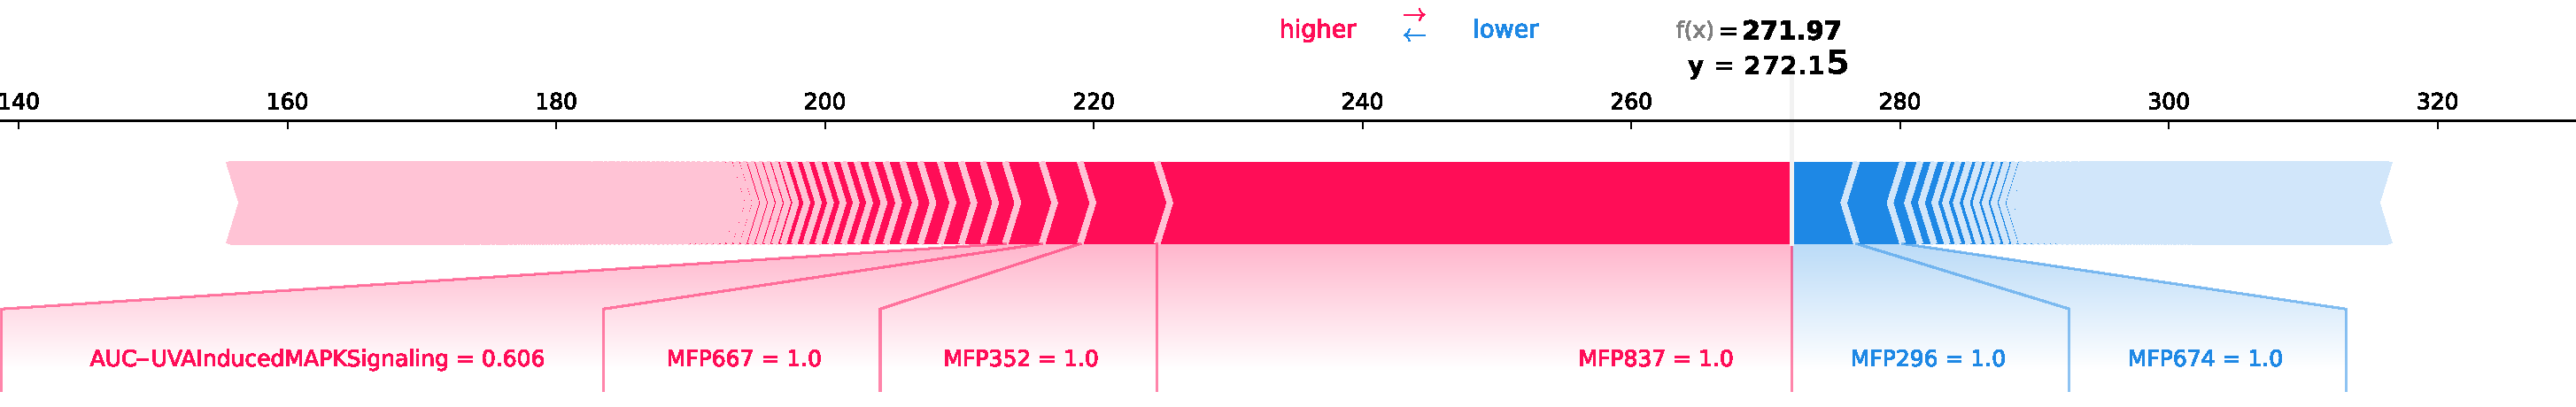
\includegraphics[width=0.80\textwidth]{jtrm_images/CatBoost_SHAP_sensitive_sample1.pdf}
    }
    \qquad
    \subfloat[Sensitive Sample 2][SHAP waterfall for a second drug-sensitive patient--drug pair.]{
        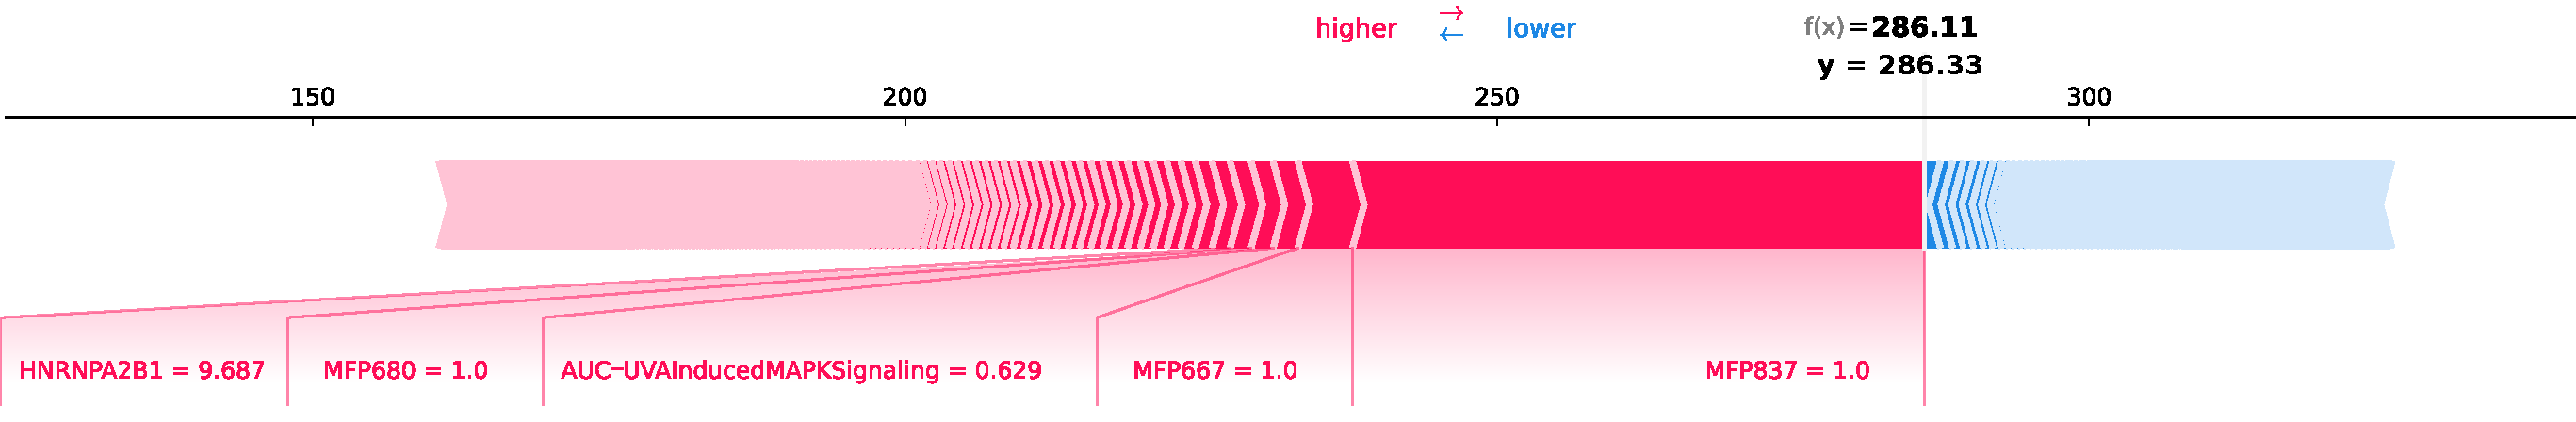
\includegraphics[width=0.80\textwidth]{jtrm_images/CatBoost_SHAP_sensitive_sample2.pdf}
    }
    \qquad
    \subfloat[Resistant Sample 1][SHAP waterfall for a drug-resistant patient--drug pair (low predicted AUC).]{
        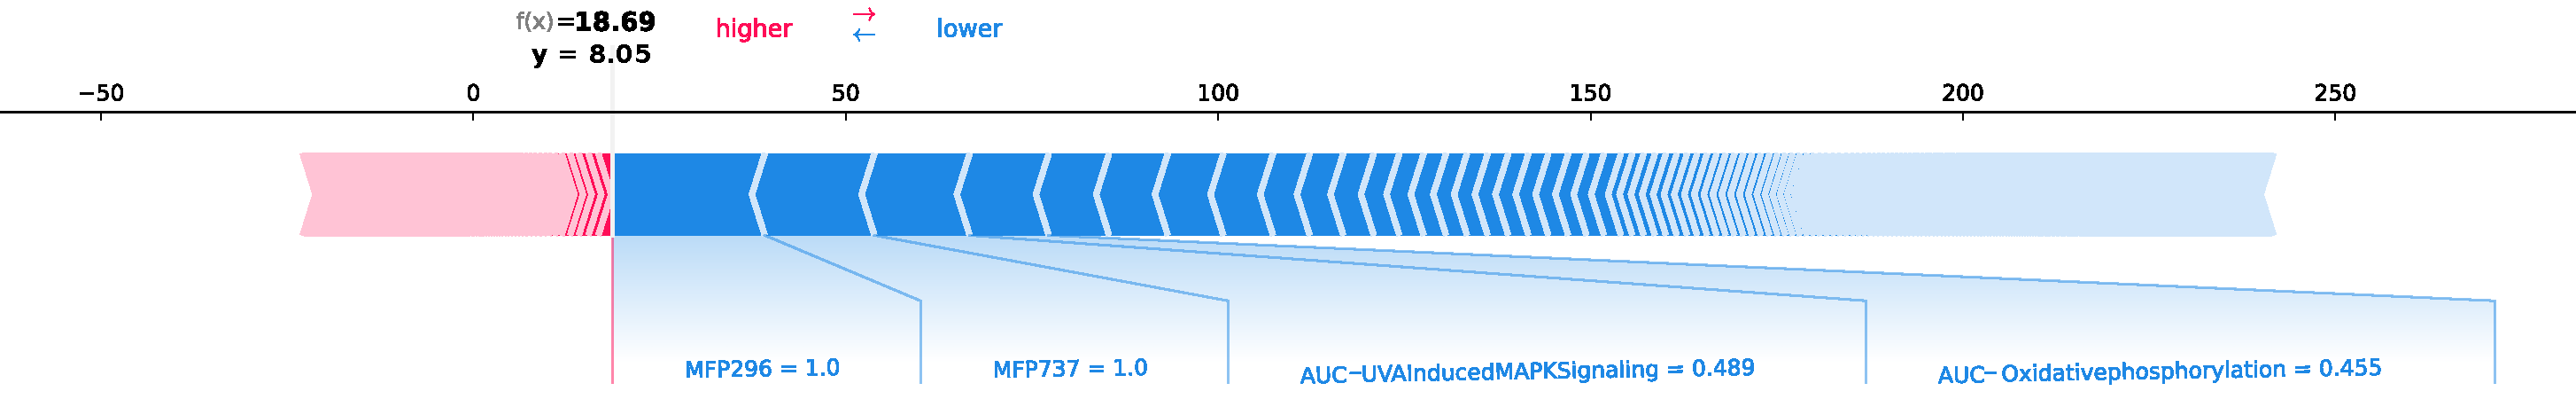
\includegraphics[width=0.80\textwidth]{jtrm_images/CatBoost_SHAP_resistance_sample1.pdf}
    }
    \qquad
    \subfloat[Resistant Sample 2][SHAP waterfall for a second drug-resistant patient--drug pair.]{
        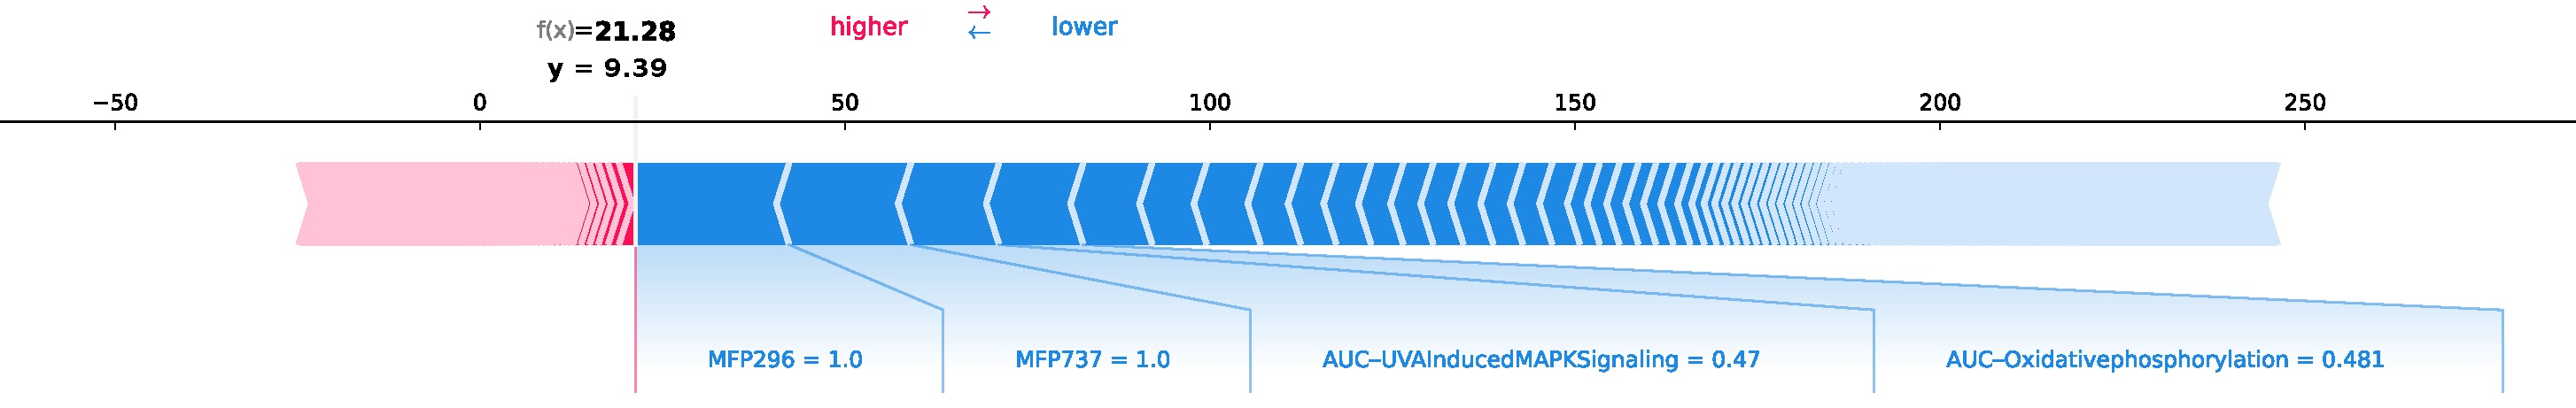
\includegraphics[width=0.80\textwidth]{jtrm_images/CatBoost_SHAP_resistance_sample2.pdf}
    }
    \caption{\textbf{CatBoost SHAP waterfall plots for representative sensitive and resistant patient--drug pairs.}
    Each bar shows the contribution of a single feature to the deviation from the baseline expected AUC.
    Features in red push the prediction toward sensitivity; features in blue push it toward resistance.}
    \label{fig:suppfig12}
\end{figure}

%% ──────────────────────────────────────────────────────────────────────────
\clearpage
\section*{Supplementary Tables}

%% Table S1 ─ Only_PC drug feature enumeration (referenced from Section 2.5)
\begin{table}[!ht]
\centering
\caption{Complete enumeration of engineered drug features comprising the
\texttt{PC} representation. Features are derived from RDKit molecular
descriptors, NetworkX graph-theoretic properties, Morgan circular fingerprints
(radius~3, 128~bits), and MACCS structural keys (167~bits). Total: 473 features.}
\label{tab:drug_features_supp}
\scriptsize
\begin{tabular}{lrr}
\toprule
\textbf{Feature Name} & \textbf{Count} & \textbf{Type} \\
\midrule
MaxAbsEStateIndex        & 1   & Descriptor \\
MinAbsEStateIndex        & 1   & Descriptor \\
MinEStateIndex           & 1   & Descriptor \\
qed                      & 1   & Descriptor \\
SPS                      & 1   & Descriptor \\
MolWt                    & 1   & Physico-chemical \\
FpDensityMorgan1         & 1   & Descriptor \\
AvgIpc                   & 1   & Descriptor \\
BalabanJ                 & 1   & Descriptor \\
Ipc                      & 1   & Descriptor \\
Kappa2                   & 1   & Descriptor \\
PEOE\_VSA                & 14  & Descriptor \\
SMR\_VSA                 & 10  & Descriptor \\
SlogP\_VSA               & 12  & Descriptor \\
TPSA                     & 1   & Descriptor \\
EState\_VSA              & 11  & Descriptor \\
VSA\_EState              & 10  & Descriptor \\
NHOHCount                & 1   & Physico-chemical \\
NumAliphaticCarbocycles  & 1   & Physico-chemical \\
NumAliphaticHeterocycles & 1   & Physico-chemical \\
NumAliphaticRings        & 1   & Physico-chemical \\
NumAmideBonds            & 1   & Physico-chemical \\
NumAromaticHeterocycles  & 1   & Physico-chemical \\
NumAtomStereoCenters     & 1   & Physico-chemical \\
NumBridgeheadAtoms       & 1   & Physico-chemical \\
NumHAcceptors            & 1   & Physico-chemical \\
NumHeteroatoms           & 1   & Physico-chemical \\
NumHeterocycles          & 1   & Physico-chemical \\
NumRotatableBonds        & 1   & Physico-chemical \\
NumSaturatedCarbocycles  & 1   & Physico-chemical \\
NumSaturatedHeterocycles & 1   & Physico-chemical \\
NumSaturatedRings        & 1   & Physico-chemical \\
NumSpiroAtoms            & 1   & Physico-chemical \\
NumUnspecifiedAtomStereoCenters & 1 & Physico-chemical \\
RingCount                & 1   & Physico-chemical \\
MolLogP                  & 1   & Physico-chemical \\
Fraction of Functional Groups & 62 & Physico-chemical \\
graph\_diameter          & 1   & Graphical \\
avg\_shortest\_path      & 1   & Graphical \\
num\_cycles              & 1   & Graphical \\
num\_chains              & 1   & Graphical \\
clustering\_coefficients & 1   & Graphical \\
avg\_degree\_centrality  & 1   & Graphical \\
avg\_eigen\_centrality   & 1   & Graphical \\
avg\_betweenness\_centrality & 1 & Graphical \\
avg\_load\_centrality    & 1   & Graphical \\
wiener\_index            & 1   & Graphical \\
max\_degree              & 1   & Graphical \\
closeness\_mean          & 1   & Graphical \\
katz\_centrality\_std    & 1   & Graphical \\
betweenness\_mean        & 1   & Graphical \\
betweenness\_std         & 1   & Graphical \\
eigenvector\_mean        & 1   & Graphical \\
rings                    & 5   & Graphical \\
heteroatom\_ratio        & 1   & Graphical \\
num\_aromatic\_rings     & 1   & Graphical \\
num\_non\_aromatic\_rings & 1  & Graphical \\
average\_atoms (C, O, S, N) & 4 & Graphical \\
num\_single\_bonds       & 1   & Graphical \\
num\_double\_bonds       & 1   & Graphical \\
Morgan (radius=3, nBits=128) & 128 & Fingerprint \\
MACCS (nBits=167)        & 167 & Fingerprint \\
\midrule
\textbf{Total}           & \textbf{473} & \\
\bottomrule
\end{tabular}
\end{table}

%% Table S2 ─ Full ML/DL benchmark
\begin{table}[!ht]
\centering
\caption{\textbf{Full benchmark of machine learning and deep learning models on the BeatAML held-out test set
(Waves~3+4, $n = 183$ samples).}
Models are grouped by class. For tree-based and linear models, the best configuration of patient feature set
and drug representation is reported. Deep learning models process drug SMILES directly.
The bold CatBoost row is the best classical model; it serves as the reference baseline for comparison with
PREDICT-AML (TabPFN).
PREDICT-AML (TabPFN) results are reported as 5-fold patient-stratified CV (PS-CV) means $\pm$ std on the
BeatAML training set (the clinically meaningful benchmark; see main text).}
\label{table:suppS1}
\resizebox{\textwidth}{!}{
\begin{tabular}{llccccc}
\toprule
\textbf{Model} & \textbf{Class} & \textbf{CV MAE} & \textbf{Test MAE} & \textbf{Test RMSE} & \textbf{Test r} & \textbf{Test R$^2$}\\
\midrule
GLR & Linear & -- & $\approx\!44.8$ & -- & $\approx\!0.55$ & -- \\
SVR & Linear & -- & $\approx\!43.1$ & -- & $\approx\!0.58$ & -- \\
\midrule
Random Forest (RF) & Tree ensemble & -- & $\approx\!42.0$ & -- & $\approx\!0.60$ & -- \\
XGBoost & Tree ensemble & -- & $\approx\!40.5$ & -- & $\approx\!0.63$ & -- \\
LightGBM & Tree ensemble & -- & $\approx\!40.8$ & -- & $\approx\!0.63$ & -- \\
\textbf{CatBoost} & \textbf{Tree ensemble} & \textbf{--} & $\mathbf{39.04}$ & $\mathbf{52.03}$ & $\mathbf{0.66}$ & $\mathbf{0.44}$ \\
\midrule
FFNN & Neural network & $18.19 \pm 1.05$ & $42.65$ & -- & $0.60$ & -- \\
\midrule
CNN & Deep learning (SMILES) & -- & $\approx\!40.85$ & -- & $\approx\!0.63$ & -- \\
LSTM & Deep learning (SMILES) & -- & $\approx\!40.70$ & -- & $\approx\!0.62$ & -- \\
GAT & Deep learning (graph) & -- & $\approx\!40.80$ & -- & $\approx\!0.63$ & -- \\
GCN & Deep learning (graph) & -- & $\approx\!40.75$ & -- & $\approx\!0.63$ & -- \\
\midrule
\multicolumn{7}{l}{\textit{PREDICT-AML TabPFN --- 5-fold patient-stratified CV on BeatAML training set}} \\
\midrule
TabPFN (Only\_PC)    & Transformer & -- & $31.790 \pm 1.451$ & $43.513 \pm 2.963$ & $0.712 \pm 0.021$ & $0.508 \pm 0.029$ \\
TabPFN (SMILES-LS)   & Transformer & -- & $31.453 \pm 0.959$ & $43.181 \pm 1.526$ & $0.716 \pm 0.013$ & $0.512 \pm 0.019$ \\
TabPFN (ChemBERTa)   & Transformer & -- & $31.574 \pm 1.417$ & $43.230 \pm 1.860$ & $0.715 \pm 0.022$ & $0.512 \pm 0.032$ \\
\textbf{TabPFN (MolFormer)} & \textbf{Transformer} & \textbf{--} & $\mathbf{31.592 \pm 1.327}$ & $\mathbf{43.138 \pm 2.793}$ & $\mathbf{0.716 \pm 0.024}$ & $\mathbf{0.513 \pm 0.034}$ \\
\bottomrule
\end{tabular}
}
\end{table}

%% Table S2 ─ TabPFN ablation results
\begin{table}[!ht]
\centering
\caption{\textbf{TabPFN feature group ablation study on BeatAML: patient-stratified CV (PS-CV) and
drug-stratified CV (DS-CV) results.}
Feature groups: \textit{Gene\_Expr} = 150 most variable genes + oncogene expression profiles;
\textit{Mutation} = somatic mutation frequency and type for top mutated genes;
\textit{Pathway} = GSVA-derived oncogenic pathway enrichment scores;
\textit{Clin\_Cell\_Mod} = clinical annotations, cell-state enrichment, and module enrichment scores.
\textit{Baseline} uses all four feature groups combined.
Results are shown for Only\_PC and SMILES-LS (Embed) drug representations under PS-CV and DS-CV.
The complete table covering all feature combinations, all three CV strategies, and all four drug
representations is available in the accompanying dataset.}
\label{table:suppS2}
\resizebox{\textwidth}{!}{
\begin{tabular}{llcccc}
\toprule
\multirow{2}{*}{\textbf{Feature Group(s)}} & \multirow{2}{*}{\textbf{Drug Rep.}} &
\multicolumn{2}{c}{\textbf{PS-CV (primary benchmark)}} & \multicolumn{2}{c}{\textbf{DS-CV}} \\
\cmidrule(lr){3-4}\cmidrule(lr){5-6}
& & \textbf{MAE} & \textbf{r} & \textbf{MAE} & \textbf{r} \\
\midrule
\textbf{Baseline (all groups)} & Only\_PC  & $31.465 \pm 1.273$ & $0.719 \pm 0.015$ & $45.804 \pm 4.371$ & $0.342 \pm 0.069$ \\
\textbf{Baseline (all groups)} & Embed     & $31.054 \pm 0.742$ & $0.724 \pm 0.015$ & $46.344 \pm 4.898$ & $0.312 \pm 0.059$ \\
\midrule
Gene\_Expr only          & Only\_PC  & $31.552 \pm 1.995$ & $0.717 \pm 0.038$ & $45.876 \pm 3.722$ & $0.335 \pm 0.043$ \\
Gene\_Expr only          & Embed     & $31.376 \pm 1.362$ & $0.718 \pm 0.023$ & $47.166 \pm 4.395$ & $0.291 \pm 0.086$ \\
\midrule
Mutation only            & Only\_PC  & $34.675 \pm 2.152$ & $0.658 \pm 0.024$ & $47.827 \pm 2.068$ & $0.237 \pm 0.062$ \\
Mutation only            & Embed     & $34.553 \pm 1.328$ & $0.659 \pm 0.023$ & $47.989 \pm 5.262$ & $0.252 \pm 0.107$ \\
\midrule
Pathway only             & Only\_PC  & $33.179 \pm 1.827$ & $0.691 \pm 0.028$ & $45.831 \pm 3.183$ & $0.331 \pm 0.021$ \\
Pathway only             & Embed     & $32.916 \pm 1.116$ & $0.694 \pm 0.025$ & $46.953 \pm 3.684$ & $0.314 \pm 0.026$ \\
\midrule
Clin\_Cell\_Mod only     & Only\_PC  & $32.499 \pm 0.427$ & $0.699 \pm 0.009$ & $46.791 \pm 1.249$ & $0.315 \pm 0.045$ \\
Clin\_Cell\_Mod only     & Embed     & $32.706 \pm 0.766$ & $0.699 \pm 0.008$ & $46.986 \pm 2.796$ & $0.314 \pm 0.040$ \\
\midrule
Gene\_Expr + Mutation    & Only\_PC  & $31.480 \pm 0.982$ & $0.716 \pm 0.023$ & $45.051 \pm 1.959$ & $0.373 \pm 0.046$ \\
Gene\_Expr + Mutation    & Embed     & $31.210 \pm 1.213$ & $0.721 \pm 0.017$ & $46.915 \pm 5.136$ & $0.314 \pm 0.070$ \\
\midrule
Gene\_Expr + Pathway     & Only\_PC  & $31.483 \pm 0.670$ & $0.718 \pm 0.010$ & $46.782 \pm 4.504$ & $0.318 \pm 0.055$ \\
Gene\_Expr + Pathway     & Embed     & $31.300 \pm 1.906$ & $0.722 \pm 0.026$ & $46.765 \pm 4.486$ & $0.318 \pm 0.077$ \\
\midrule
Clin\_Cell\_Mod + Mutation & Only\_PC & $32.293 \pm 2.316$ & $0.702 \pm 0.031$ & $45.031 \pm 1.963$ & $0.378 \pm 0.023$ \\
Clin\_Cell\_Mod + Mutation & Embed    & $32.639 \pm 1.948$ & $0.697 \pm 0.027$ & $47.898 \pm 4.491$ & $0.277 \pm 0.041$ \\
\midrule
Clin\_Cell\_Mod + Gene\_Expr & Only\_PC & $31.524 \pm 1.461$ & $0.716 \pm 0.018$ & $45.997 \pm 2.153$ & $0.317 \pm 0.049$ \\
Clin\_Cell\_Mod + Gene\_Expr & Embed   & $31.128 \pm 1.500$ & $0.720 \pm 0.026$ & $46.658 \pm 4.367$ & $0.322 \pm 0.133$ \\
\midrule
Clin\_Cell\_Mod + Gene\_Expr + Mutation & Only\_PC & $31.606 \pm 1.831$ & $0.718 \pm 0.022$ & $45.116 \pm 3.535$ & $0.364 \pm 0.029$ \\
Clin\_Cell\_Mod + Gene\_Expr + Mutation & Embed   & $31.096 \pm 2.222$ & $0.725 \pm 0.031$ & $46.658 \pm 2.626$ & $0.308 \pm 0.085$ \\
\midrule
Clin\_Cell\_Mod + Mutation + Pathway & Only\_PC & $32.161 \pm 1.183$ & $0.705 \pm 0.008$ & $45.242 \pm 4.352$ & $0.396 \pm 0.047$ \\
Clin\_Cell\_Mod + Mutation + Pathway & Embed    & $32.068 \pm 2.150$ & $0.709 \pm 0.040$ & $47.050 \pm 3.600$ & $0.288 \pm 0.041$ \\
\bottomrule
\end{tabular}
}
\end{table}

\end{document}

